\documentclass[11pt,letter]{article}
\usepackage[top=1.00in, bottom=1.0in, left=1.1in, right=1.1in]{geometry}
\renewcommand{\baselinestretch}{1.6}
\usepackage{graphicx}
\usepackage{natbib}
\usepackage{amsmath}
\usepackage{amssymb} 

\def\labelitemi{--}
\parindent=0pt
\begin{document}


{\bf Graphical asbtract} for: A simple explanation for declining temperature sensitivity with warming (E. M. Wolkovich,  J. L. Auerbach, C. J. Chamberlain, D. M. Buonaiuto, A. K. Ettinger, I. Morales-Castilla \& A. Gelman)\\

Recently a growing body of literature has used shifting phenological sensitivities with higher temperatures as evidence that climate change is already reshaping fundamental biological processes. Here we show that these results may simply be the outcome of using linear models (left) to estimate non-linear temperature responses, specifically for events that occur after a cumulative thermal threshold is met---a common model for many biological events. Corrections for the non-linearity of temperature responses consistently remove the apparent decline (right). Our results suggest that current methods may undermine efforts to identify when and how warming will reshape biological processes.\\

\begin{figure}[h!]
\centering
\noindent 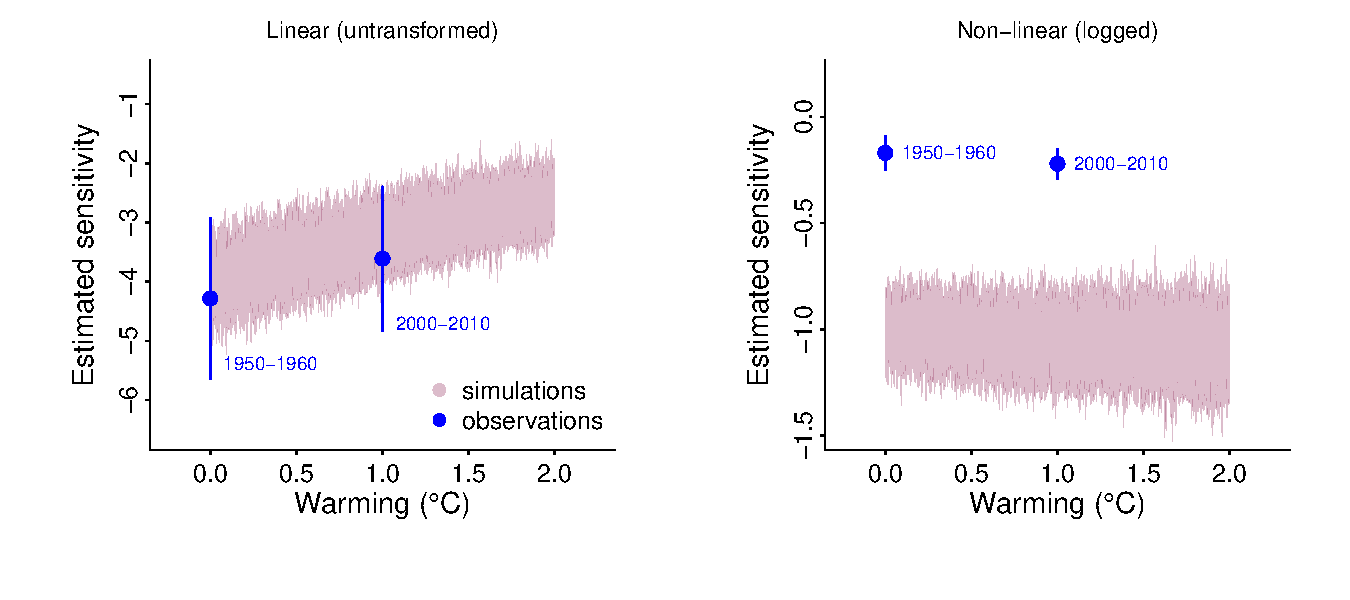
\includegraphics[width=1.05\textwidth]{..//analyses/figures/basicsimsandpepalt1.pdf} 
\end{figure}

\end{document}
